%\section{Scientific Visualization}
\subsection{Generalities}
\begin{frame}
    \frametitle{Scientific Visualization}
    \framesubtitle{}

    \vspace{-2.5mm}
    \begin{columns} %[T]
    \begin{column}{5.325cm}
        \begin{itemize}
                \item represent data
                \item plotting
                \item visualization techniques
                \item analyze/explore
                \item communicate (publications/talks)
                \item make it look nice?
        \end{itemize}

        \centering
        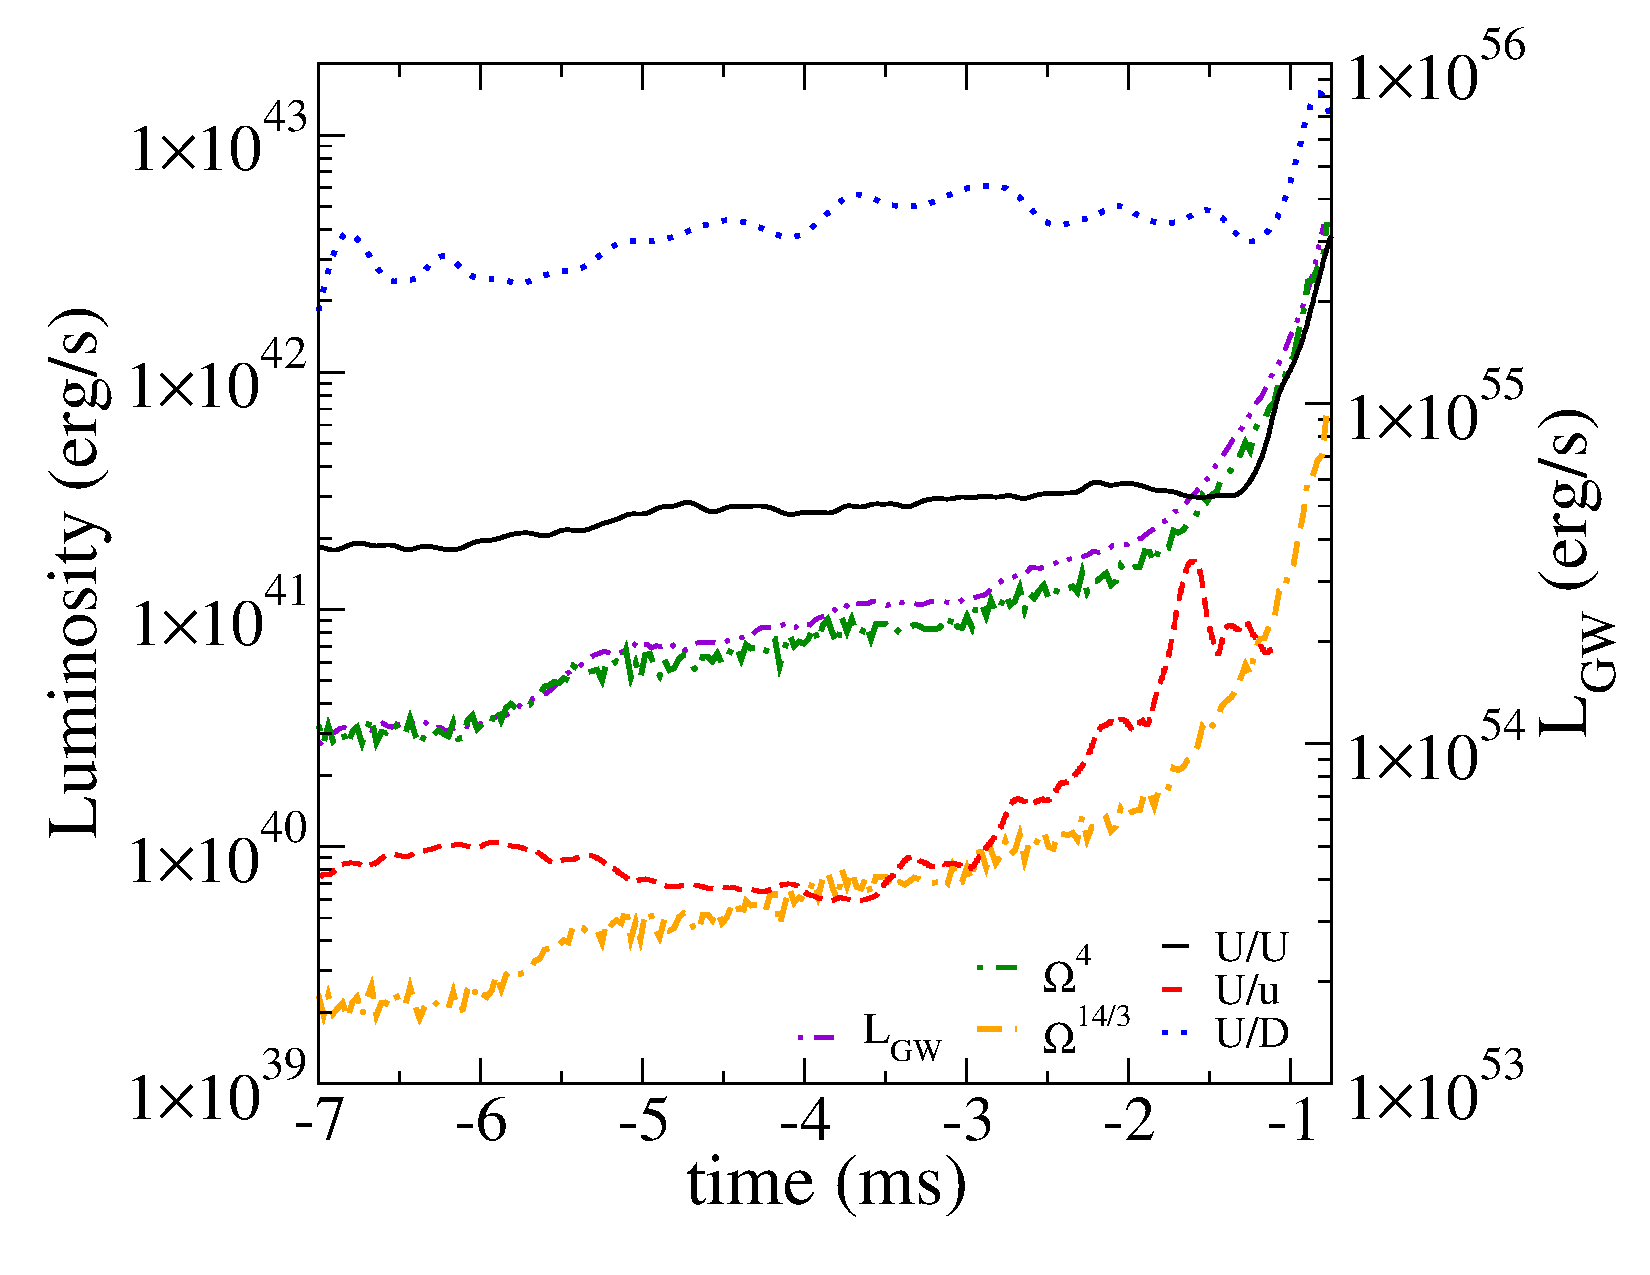
\includegraphics[width=.5\columnwidth]{figs/plots/mpc/figure3_B}

        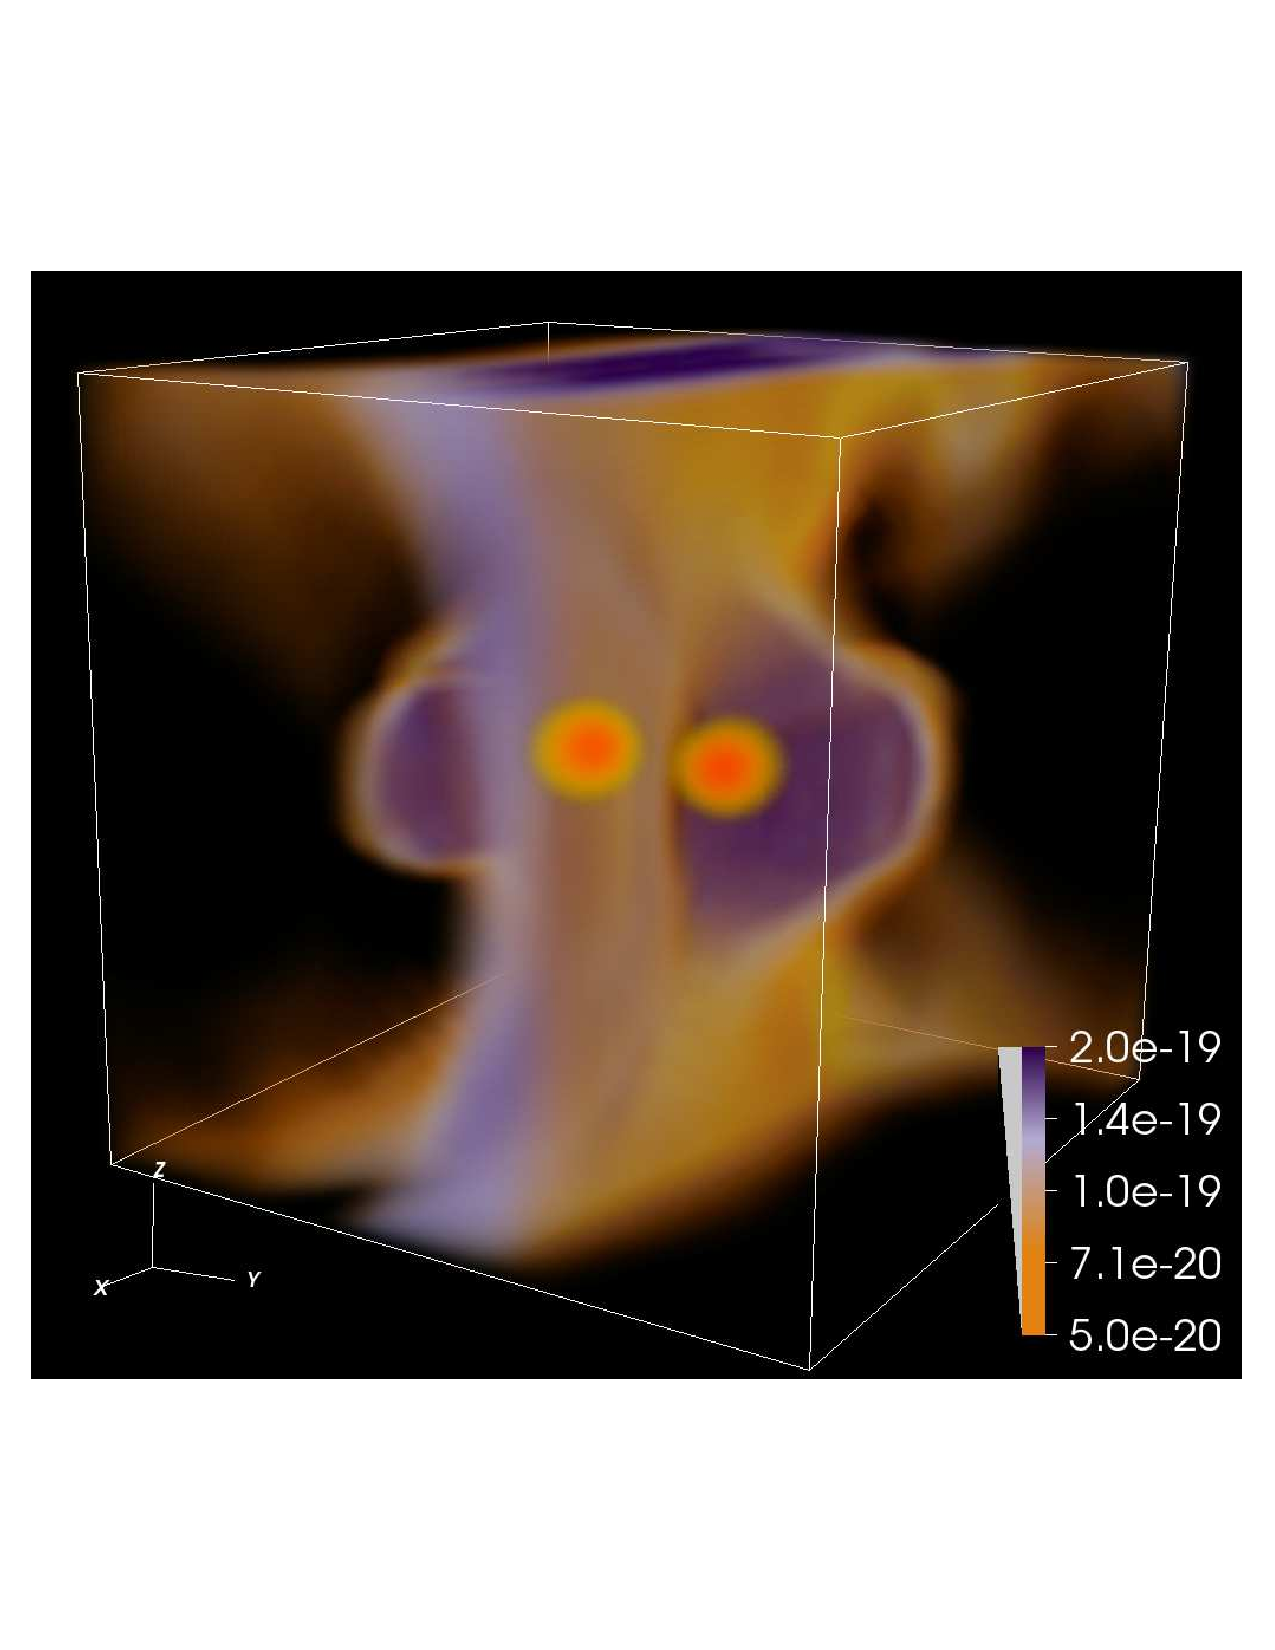
\includegraphics[width=0.33\columnwidth]{figs/plots/mpc/bns01_UU-sqphi2_3d-14b}
        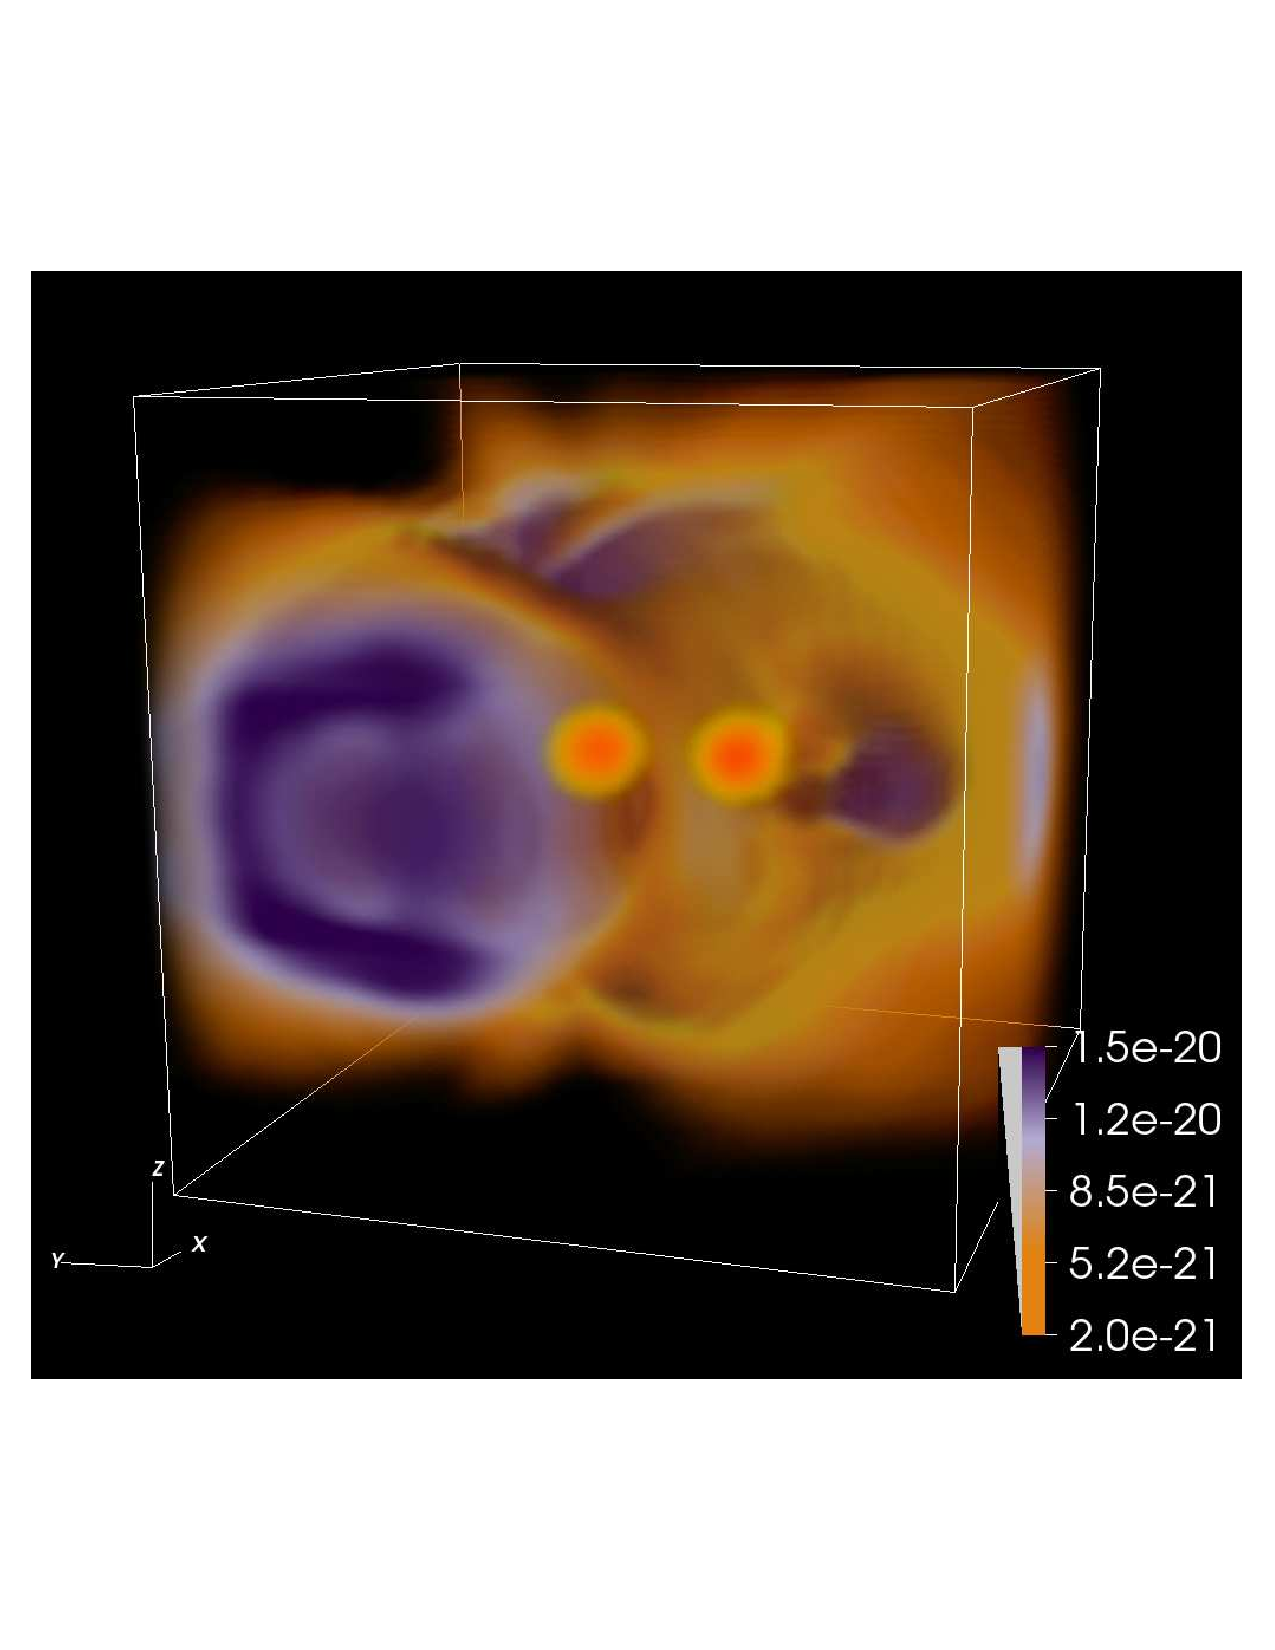
\includegraphics[width=0.33\columnwidth]{figs/plots/mpc/bns02_Uu-sqphi2_3d-14c}
        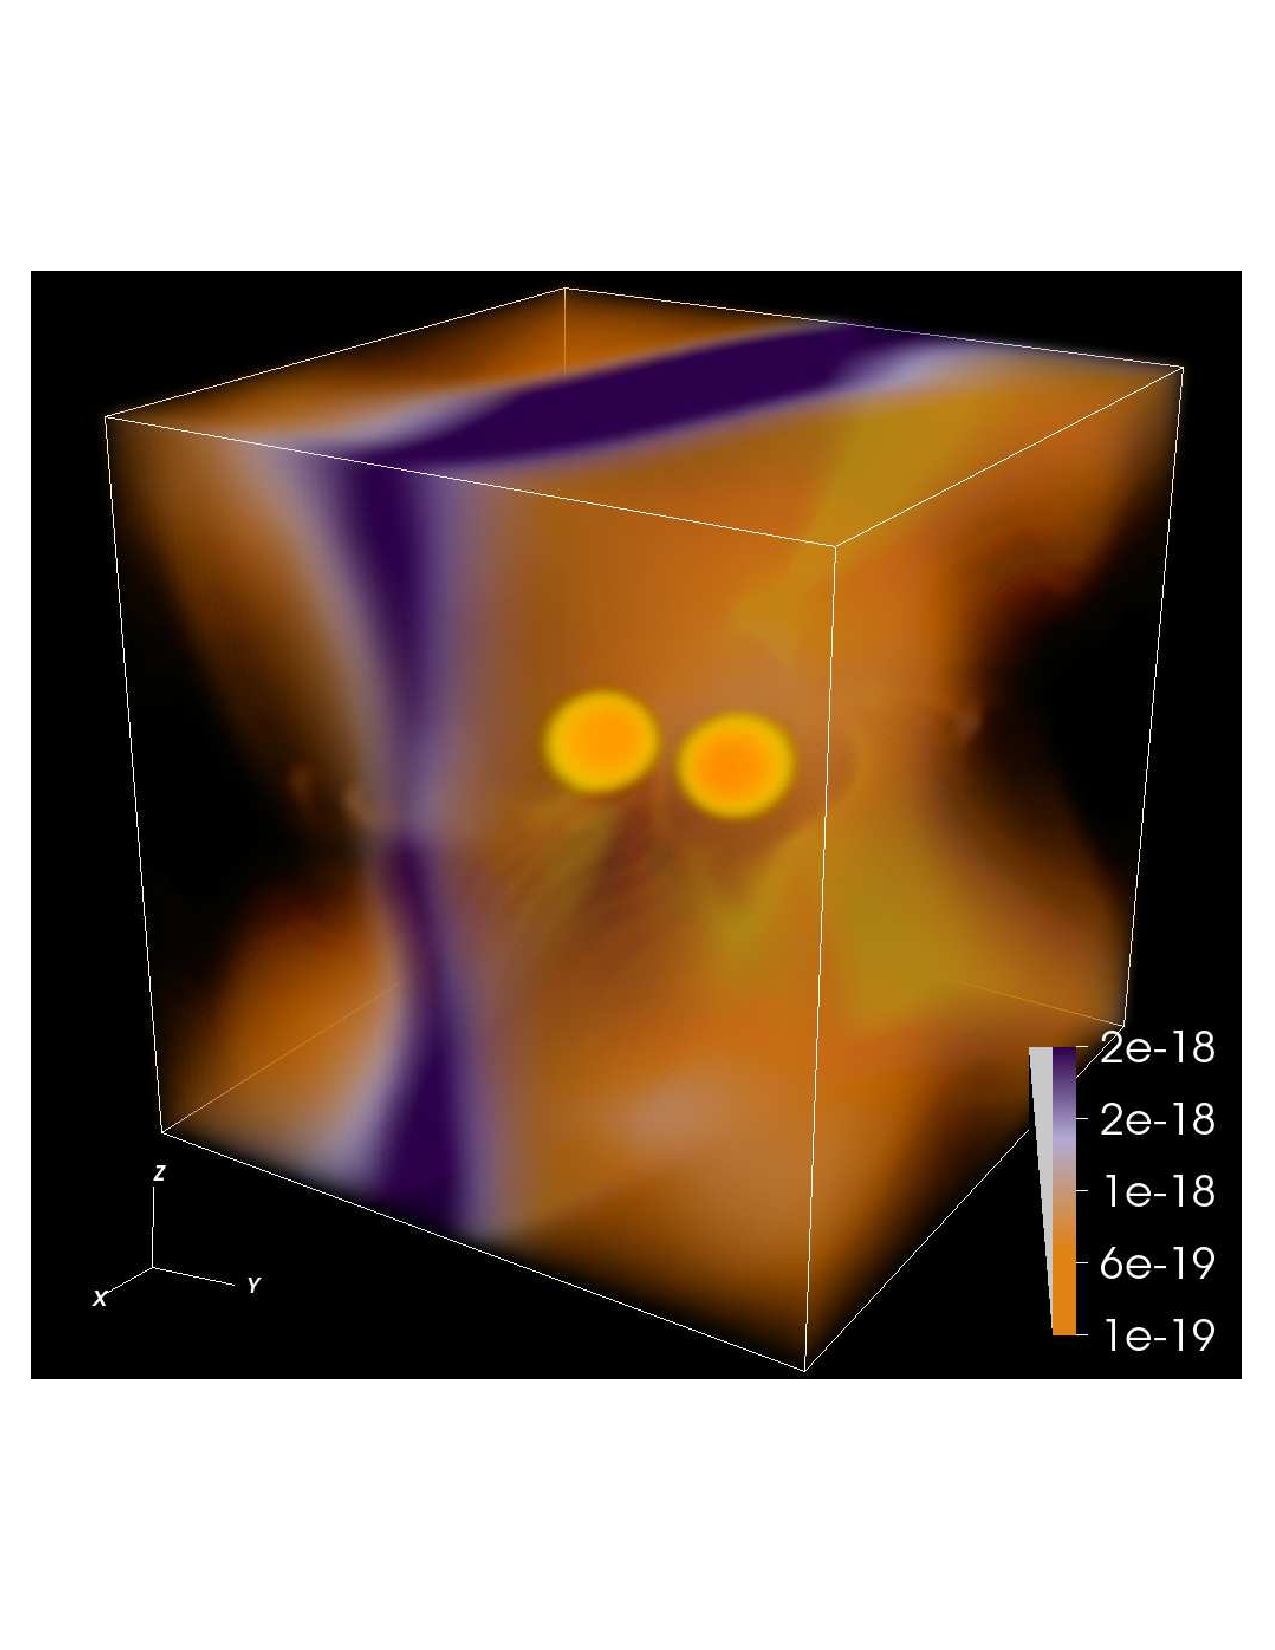
\includegraphics[width=0.33\columnwidth]{figs/plots/mpc/bns03_UD-sqphi2_3d-14b}
    \end{column}
    \begin{column}{7.5cm}
        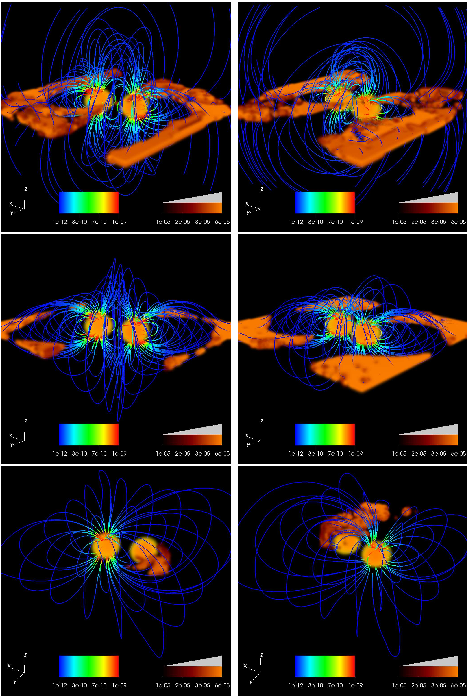
\includegraphics[width=\columnwidth,clip=true,trim=0 4cm 0 4cm]{figs/plots/mpc/plot_Bxi}
        %
        %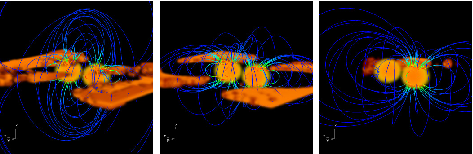
\includegraphics[width=\columnwidth]{figs/plots/mpc/figure1_c}
        \\
        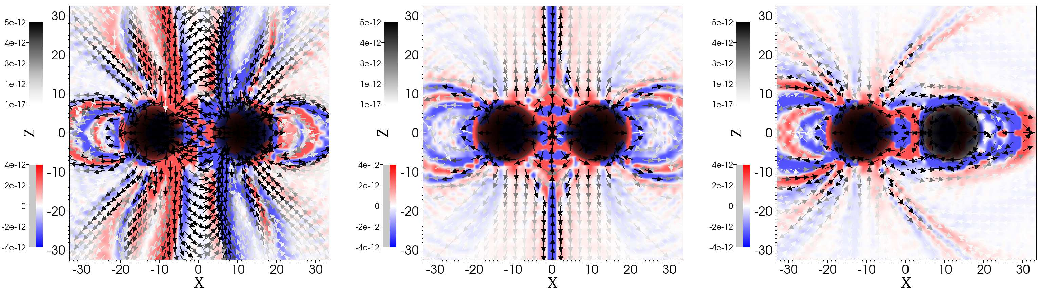
\includegraphics[width=\columnwidth]{figs/plots/mpc/plot_current}
        \\
        %\href{http://journals.aps.org/prd/kaleidoscope/}{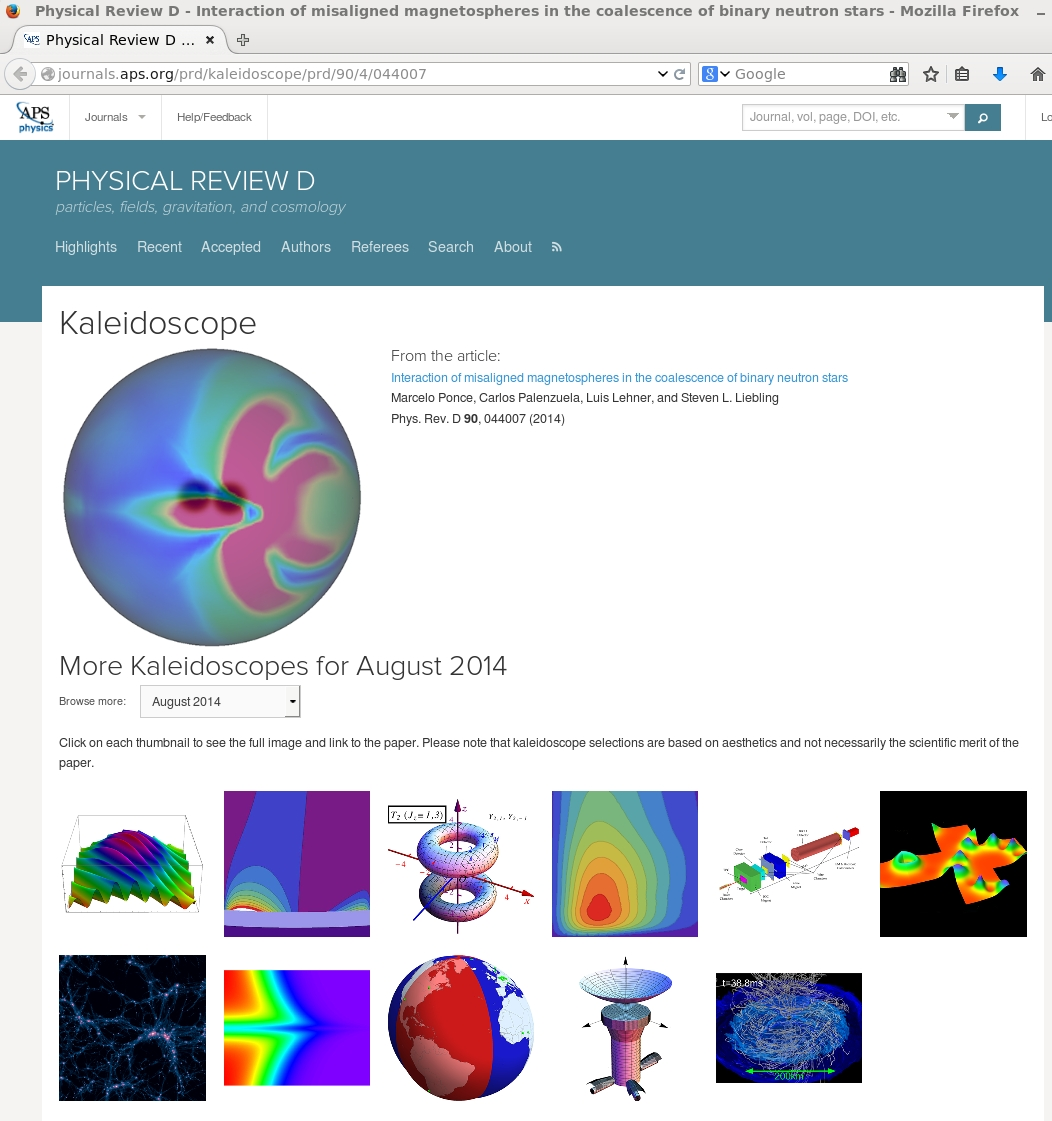
\includegraphics[width=\columnwidth, clip=true,trim=1.25cm 3.5mm 3.5mm 19.75cm]{figs/plots/mpc/kaleidoscope}
        \href{http://journals.aps.org/prd/kaleidoscope/August2014}{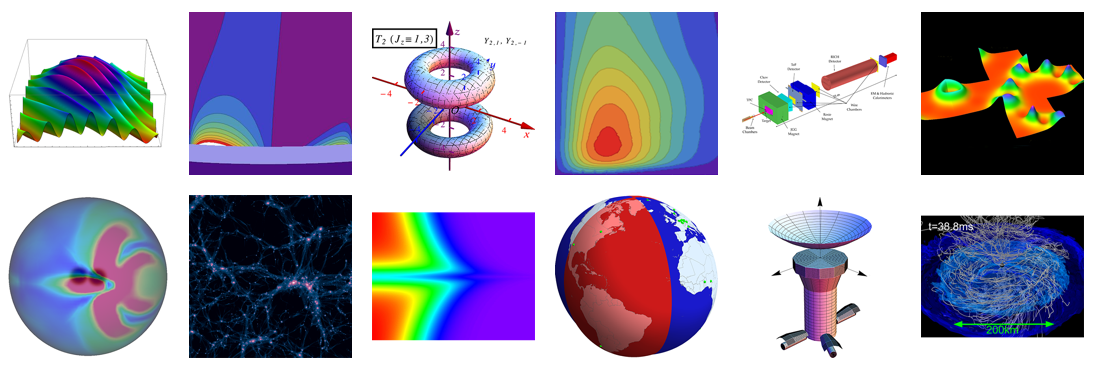
\includegraphics[width=\columnwidth]{figs/plots/mpc/kaleidoscope_aug2014}}
    \end{column}
    \end{columns}
\end{frame}


\subsection{2D/3D Visualization Generalities}
\begin{frame}
    \frametitle{}
    \framesubtitle{}

    \begin{columns} %[T]
    \begin{column}{5.25cm}
        \begin{itemize}
                \item \textcolor{DarkBlue}{Visualization} is the process of mapping (scientific) data into ``{\it visual form}''
                \item Much easier to understand images than a large set of numbers
                \item For interactive data exploration, debugging, communication with peers
        \end{itemize}
    \end{column}
    \begin{column}{7cm}
        \href{http://www.paraview.org/gallery/}{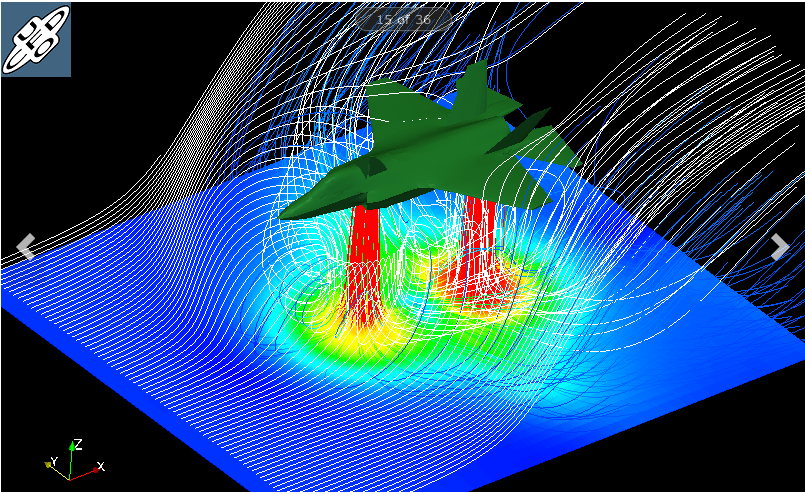
\includegraphics[width=.475\columnwidth]{figs/paraview/ParaView-gallery01}}
        \href{http://www.paraview.org/gallery/}{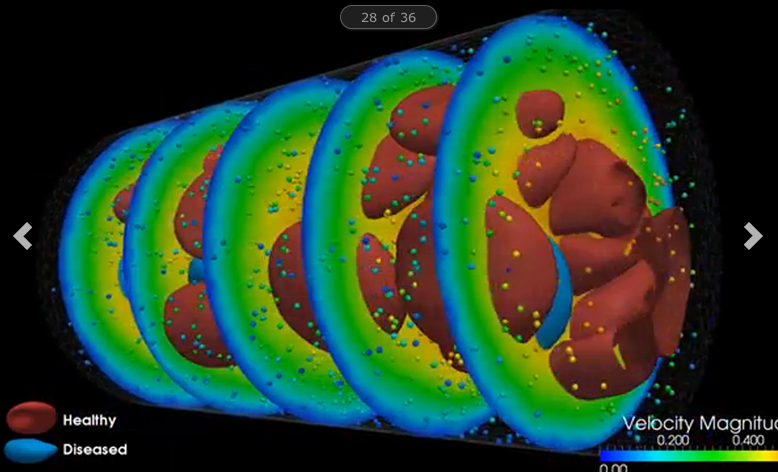
\includegraphics[width=.475\columnwidth]{figs/paraview/ParaView-gallery03}}
        \centering
        \href{http://www.paraview.org}{
\includegraphics[width=.45\columnwidth]{./figs/visit-logos/ParaViewLogo}}


        \href{https://wci.llnl.gov/simulation/computer-codes/visit/gallery}{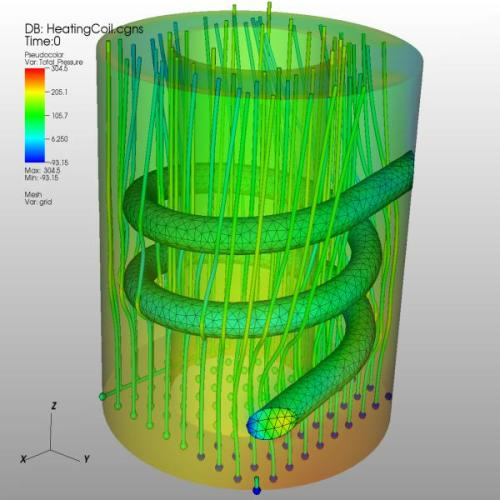
\includegraphics[width=.475\columnwidth]{figs/visit-exs/VisIt-gallery_12}}
        \href{https://wci.llnl.gov/simulation/computer-codes/visit/gallery}{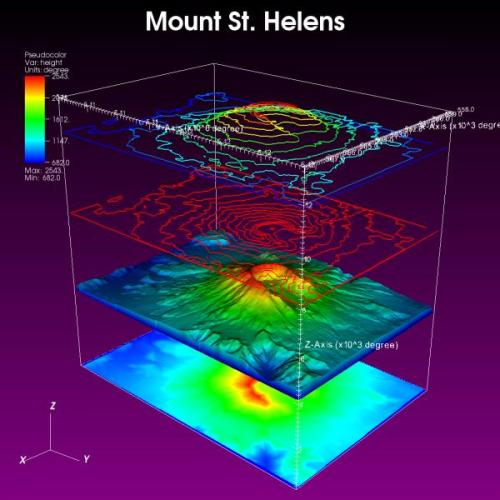
\includegraphics[width=.475\columnwidth]{figs/visit-exs/VisIt-gallery_15}}

        \centering
        \href{https://wci.llnl.gov/simulation/computer-codes/visit/}{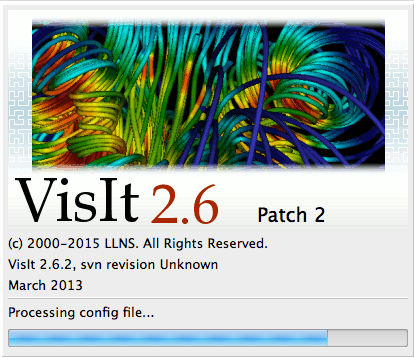
\includegraphics[width=.45\columnwidth, clip=true,trim=0 2cm 0 0]{./figs/visit-logos//VisIt26}}
    \end{column}
    \end{columns}


%    \begin{columns} %[T]
%    \begin{column}{5.5cm}
%       \centering
%       \href{https://wci.llnl.gov/simulation/computer-codes/visit/}{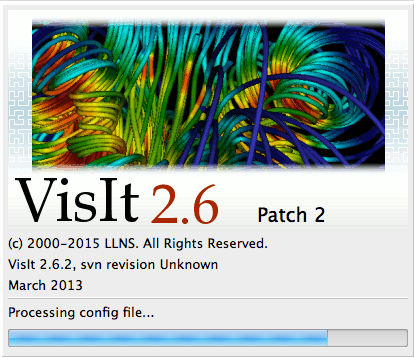
\includegraphics[width=.75\columnwidth, clip=true,trim=0 2cm 0 0]{./figs/visit-logos//VisIt26}}
%    \end{column}
%    \begin{column}{5.5cm}
%       \centering
%       \href{http://www.paraview.org}{
\includegraphics[width=.7\columnwidth]{./figs/visit-logos//ParaViewLogo}}
%    \end{column}
%    \end{columns}

\end{frame}


\begin{frame}
\frametitle{1D plotting vs. 2D/3D visualization}

\begin{columns}
\begin{column}{7cm}
\begin{beamerboxesrounded}[upper=block head,lower=block body,shadow=true]{\textcolor{DarkBlue}{\ding{232}} \textcolor{DarkGreen}{1D plotting}}
         plotting functions of one variable, 1D tabulated data (eg. \textcolor{DarkBlue}{\tt gnuplot},  \textcolor{DarkBlue}{\tt xmgr}, or Python's \textcolor{DarkRed}{\tt matplotlib} library)
\end{beamerboxesrounded}
\end{column}
\begin{column}{5cm}
        \centering
        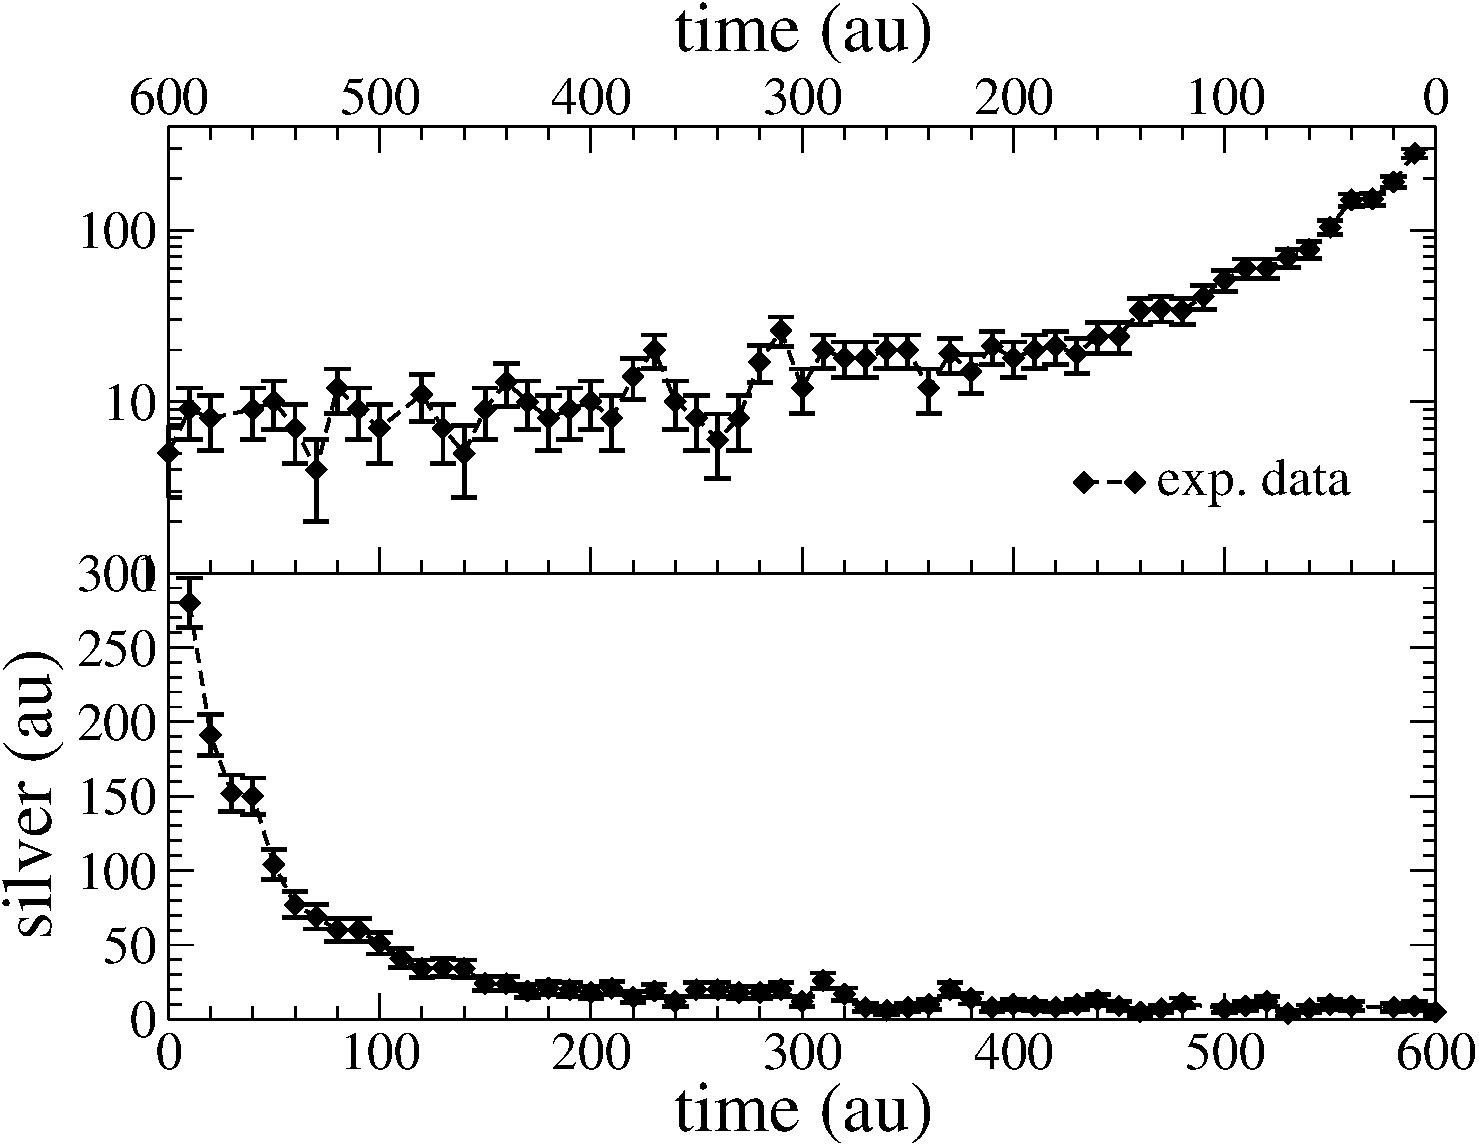
\includegraphics[width=.85\columnwidth]{figs/plots/others/silver_2plots}
\end{column}
\end{columns}

\begin{columns}
\begin{column}{7cm}
\begin{beamerboxesrounded}[upper=block head,lower=block body,shadow=true]{\textcolor{DarkBlue}{\ding{232}} \textcolor{DarkOrange}{2D/3D visualization} }
        displaying multi-dimensional datasets, typically
data on 2D/3D structured grids or on unstructured meshes (that have
some topology in 2D/3D)
\end{beamerboxesrounded}
\end{column}
\begin{column}{5cm}
        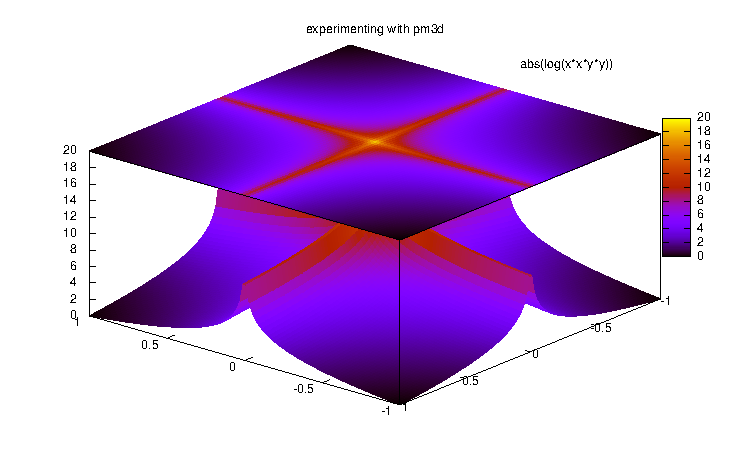
\includegraphics[width=1.1\columnwidth]{figs/plots/others/pm3dplot}
\end{column}
\end{columns}

%Whatever you do, may be a good idea to avoid proprietary tools, unless those tools provide a clear advantage (most likely not)
%\begin{itemize}
%       \item large \$\$
%       \item limitations on where you can run them, which machines/platforms, etc.
%       \item cannot get help from open-source community, user base usually smaller than for open-source tools
%       \item once you start accumulating scripts, you lock yourself into using these tools forever, and consequently paying \$\$ on a regular basis
%       \item there is nothing you cannot do with open-source tools
%\end{itemize}
\end{frame}


\begin{frame}
\frametitle{2D/3D visualization packages}

\begin{small}
\vspace{-2mm}
%\begin{beamerboxesrounded}[upper=block head,lower=block body,shadow=true]{
\textcolor{DarkRed}{\ding{232}} \textcolor{DarkBlue}{\tt gnuplot}: %}
        command-driven interactive 2d and 3d plotting program
%\end{beamerboxesrounded}

\vspace{1.15mm}
%\begin{beamerboxesrounded}[upper=block head,lower=block body,shadow=true]{
\textcolor{DarkRed}{\ding{232}} \textcolor{DarkBlue}{\tt GraphViz}: %}
        represent structural information as diagrams of abstract graphs and networks
%\end{beamerboxesrounded}

\vspace{1.15mm}
%\begin{beamerboxesrounded}[upper=block head,lower=block body,shadow=true]{
\textcolor{DarkRed}{\ding{232}} \textcolor{DarkBlue}{\tt HDFview}: %}
        visual tool for browsing and editing HDF4 and HDF5 files
%\end{beamerboxesrounded}

\vspace{1.15mm}
%\begin{beamerboxesrounded}[upper=block head,lower=block body,shadow=true]{
\textcolor{DarkRed}{\ding{232}} \textcolor{DarkBlue}{\tt ImageMagick}: %}
        manipulation of image
%\end{beamerboxesrounded}

\vspace{1.15mm}
%\begin{beamerboxesrounded}[upper=block head,lower=block body,shadow=true]{
\textcolor{DarkRed}{\ding{232}} \textcolor{DarkBlue}{\tt Molden}: %}
        pre/post-processing for molecular and electronic structures
%\end{beamerboxesrounded}

\vspace{1.15mm}
%\begin{beamerboxesrounded}[upper=block head,lower=block body,shadow=true]{
\textcolor{DarkRed}{\ding{232}} \textcolor{DarkBlue}{\tt OpenCV}: %}
        library for real time computer vision
%\end{beamerboxesrounded}

%\vspace{1.15mm}
\begin{beamerboxesrounded}[upper=block head,lower=block body,shadow=true]{}
\textcolor{DarkRed}{\ding{232}} \textcolor{DarkBlue}{\tt ParaView}: %}
        Parallel visualization application
\end{beamerboxesrounded}

%\vspace{1.15mm}
%\begin{beamerboxesrounded}[upper=block head,lower=block body,shadow=true]{
\textcolor{DarkRed}{\ding{232}} \textcolor{DarkBlue}{\tt SciLab}: %}
        open source platform for numerical computation
%\end{beamerboxesrounded}

%\vspace{1.15mm}
\begin{beamerboxesrounded}[upper=block head,lower=block body,shadow=true]{}
\textcolor{DarkRed}{\ding{232}} \textcolor{DarkBlue}{\tt VisIt}: %}
        Visualization Tool for HPC
\end{beamerboxesrounded}

%\vspace{1.15mm}
%\begin{beamerboxesrounded}[upper=block head,lower=block body,shadow=true]{
\textcolor{DarkRed}{\ding{232}} \textcolor{DarkBlue}{\tt XCrysDen}: %}
        Crystaline and Molecular Structure Visualization
%\end{beamerboxesrounded}

\vspace{1.15mm}
%\begin{beamerboxesrounded}[upper=block head,lower=block body,shadow=true]{
\textcolor{DarkRed}{\ding{232}} \textcolor{DarkBlue}{\tt yt}: %}
        python-based package for visualization of AMR datasets
%\end{beamerboxesrounded}

\vspace{1.15mm}
%\begin{beamerboxesrounded}[upper=block head,lower=block body,shadow=true]{
\textcolor{DarkRed}{\ding{232}} \textcolor{DarkBlue}{\tt VMD}: %}
        Visualization for Molecular Dynamics
%\end{beamerboxesrounded}

%\vspace{1.15mm}
%\begin{beamerboxesrounded}[upper=block head,lower=block body,shadow=true]{
\textcolor{DarkRed}{\ding{232}} \textcolor{DarkBlue}{\tt openDX}: %}
        very old, not mantained package, but really \\nice approach to visualization process (modules)
%\end{beamerboxesrounded}
\end{small}
\end{frame}


\begin{frame}
\frametitle{2D/3D visualization packages}
\framesubtitle{General Features}

\begin{itemize}
        \item visualize \textcolor{DarkBlue}{scalar} and \textcolor{DarkBlue}{vector fields}
        \item \textcolor{DarkBlue}{structured and unstructured meshes} in 2D and 3D, particle data, polygonal
data, \textcolor{DarkBlue}{irregular topologies}
        \item ability to handle very \textcolor{DarkBlue}{large datasets} (GBs to TBs)
        \item ability to scale to large ($10^3 - 10^5$ cores) computing facilities
        \item \textcolor{DarkBlue}{iteractive manipulation}
        \item support for \textcolor{DarkBlue}{scripting}, \textcolor{DarkBlue}{common data formats}, \textcolor{DarkBlue}{parallel I/O}
        \item open-source, \textcolor{DarkBlue}{multi-platform}, and \textcolor{DarkBlue}{general-purpose}
\end{itemize}

    \begin{columns} %[T]
    \begin{column}{5.5cm}
        \centering
        \href{https://wci.llnl.gov/simulation/computer-codes/visit/}{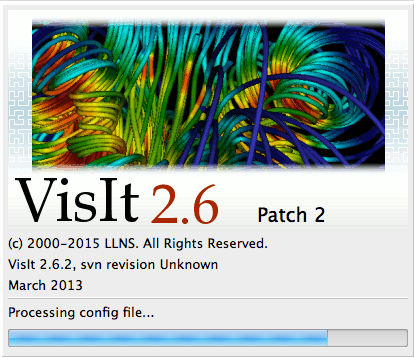
\includegraphics[width=.75\columnwidth, clip=true,trim=0 2cm 0 0]{./figs/visit-logos//VisIt26}}
    \end{column}
    \begin{column}{5.5cm}
        \centering
        \href{http://www.paraview.org}{
\includegraphics[width=.7\columnwidth]{./figs/visit-logos//ParaViewLogo}}
    \end{column}
    \end{columns}

\end{frame}



\subsection{Visualization Pipeline}
\begin{frame}

\begin{columns}
\begin{column}{8cm}
        \begin{beamerboxesrounded}[upper=block head,lower=block body,shadow=true]{\textcolor{DarkBlue}{\ding{231}} Data Visualization Process}
                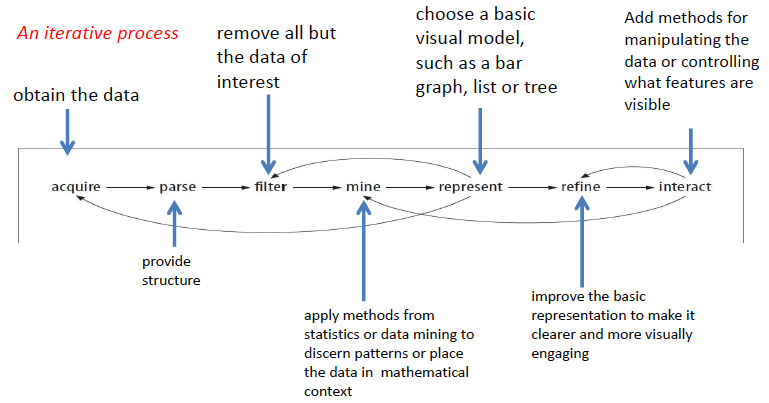
\includegraphics[width=\columnwidth]{figs/viz/viz_pipeline-loop}
        \end{beamerboxesrounded}
\end{column}
\begin{column}{4.5cm}
        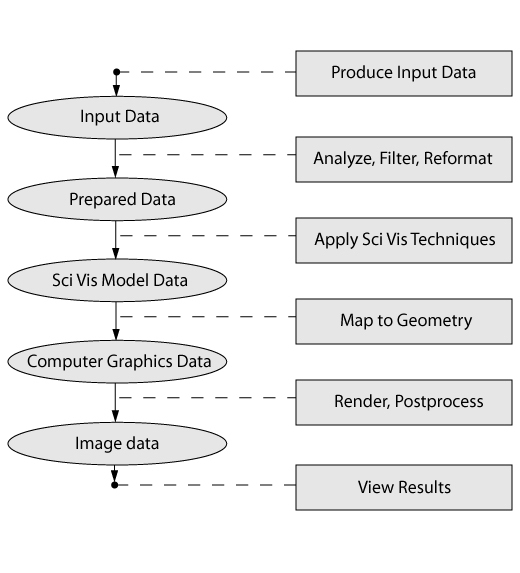
\includegraphics[width=\columnwidth]{figs/viz/viz-pipeline4}
\end{column}
\end{columns}

\begin{small}
\begin{columns}
\begin{column}{3.85cm}
\begin{beamerboxesrounded}[upper=block head,lower=block body,shadow=true]{\textcolor{DarkRed}{\ding{231}} Scientific Visualization Techniques}
        \textcolor{DarkRed}{\ding{224}} contours/isosurfaces, clips, thresholds, glyphs, streamlines, pseducolors, ...
\end{beamerboxesrounded}
\end{column}
\begin{column}{3.85cm}
\begin{beamerboxesrounded}[upper=block head,lower=block body,shadow=true]{\textcolor{DarkRed}{\ding{231}} Map to Geometry}
        \textcolor{DarkRed}{\ding{223}} scalars, vectors, tensors

        \textcolor{DarkRed}{\ding{223}} 1D, 2D, 3D

        \textcolor{DarkRed}{\ding{223}} mesh/grid
\end{beamerboxesrounded}
\end{column}
\begin{column}{3.85cm}
\begin{beamerboxesrounded}[upper=block head,lower=block body,shadow=true]{\textcolor{DarkRed}{\ding{231}} Render/PostProcess}
        \centering
        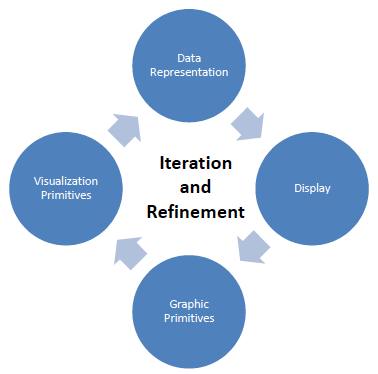
\includegraphics[width=.75\columnwidth]{figs/viz/render}
\end{beamerboxesrounded}
\end{column}
\end{columns}
\end{small}
\end{frame}



\subsection{VTK: Visualization ToolKit}

\begin{frame}
\frametitle{Visualization Toolkit (VTK) -- \url{http://www.vtk.org/}}

\begin{columns}
\begin{column}{5.75cm}
\begin{itemize}
        \item Open source, multiplatform
        \item Supports distributed computation models
        \item Extensible modular architecture
        \item Available for 3D computer graphics, image processing and visualization
        \item Collection of C++ libraries
\end{itemize}
\end{column}
\begin{column}{5.75cm}
\begin{itemize}
        \item Leveraged by many applications
        \item Divided into logical areas
                \begin{itemize}
                        \item Filtering
                        \item Information Visualization
                        \item  Volume Rendering
                \end{itemize}
        \item Cross platform, using OpenGL
        \item Wrapped in Python, Tool Command Language (Tcl) and Java
\end{itemize}
\end{column}
\end{columns}

\vspace{3.5mm}
\textcolor{DarkBlue}{\ding{231}} {\bf ParaView} and {\bf VisIt} are end-user applications with support:

\hspace{5mm}
\textcolor{DarkBlue}{\ding{223}} \textit{parallel} Data Archiving/Reading/Processing/Rendering

\hspace{5mm}
\textcolor{DarkBlue}{\ding{223}} single node, \textit{Client-Server}, \textit{MPI Cluster} Rendering
\end{frame}

